	All results shown are averaged from five trial runs with the aforementioned parameters. Table \ref{overviewResults} displays results obtained from baseline and optimized experiments alongside the results from the original experiment. Neural networks perform similarly to LDA/Cosine Similarity as a discriminant and classifier algorithm. However, when using LDA/DNN, Neural Networks perform much better due to the reduced feature size minimizing overfitting. Although (Batliner et. al 2004) achieved similar impressive results with a large feature vector, the features were carefully selected and separable beforehand. This is not the case with the 100 dimension I Vector wherein the DNN overfits, but is the case for the dimensionally reduced variant as observed by the large differential in their accuracy.
	
	As discussed earlier in the project, humans can disagree on labels. This can be observed by checking the label process of the data used. Each utterance has three labels. If only unanimous labels were used, there would only be a total of \textbf{2124} labels to use. That is only 40\% of the data; therefore if humans can only completely agree on 40\%, an automatic emotion recognition system can be expected to perform at least similarly.
	\begin{table}[ht]
		\caption{Results of Classifers with 80/20 train/test split}
			\centering
		\begin{tabular}{|c|c|c|}
			\hline
			Classifier                            & Features & UAR  \\ \hline
			Cosine Similarity                     & 5        & 24\% \\ \hline
			Euclidean Distance                     & 5        & 46\% \\ \hline
			Neural Network (Batliner et. al 2004) & 125      & 69\% \\ \hline
			DNN (Baseline)                        & 100      & 24\% \\ \hline
			LDA/DNN (Baseline)                        & 5        & 77\% \\ \hline
			LDA/DNN (Optimized)                       & 5        & 81\% \\ \hline
		\end{tabular}
	\label{overviewResults}
	\end{table}
	\section{Maximum Linear Separability of Data}
	Figure \ref{fig:5graphLDA} is the plot in all five dimensions, two dimensions at a time. Neutral, Angry and Emphatic utterances overlap in most dimensions, whereas the remainder are clearly separable in at least one dimensions. Neutral, Angry and Emphatic have the three largest samples out of the classes. This indicates the emotion of joyful, motherese or other is clearly expressed by the children despite the low number of times it is expressed, whereas the remainder have a chance to be confused with each other even by the labellers. The overlapping emotional classes could be closely matched but differ in a scale such as intensity.
	
		\begin{figure}[!htb]
		\center{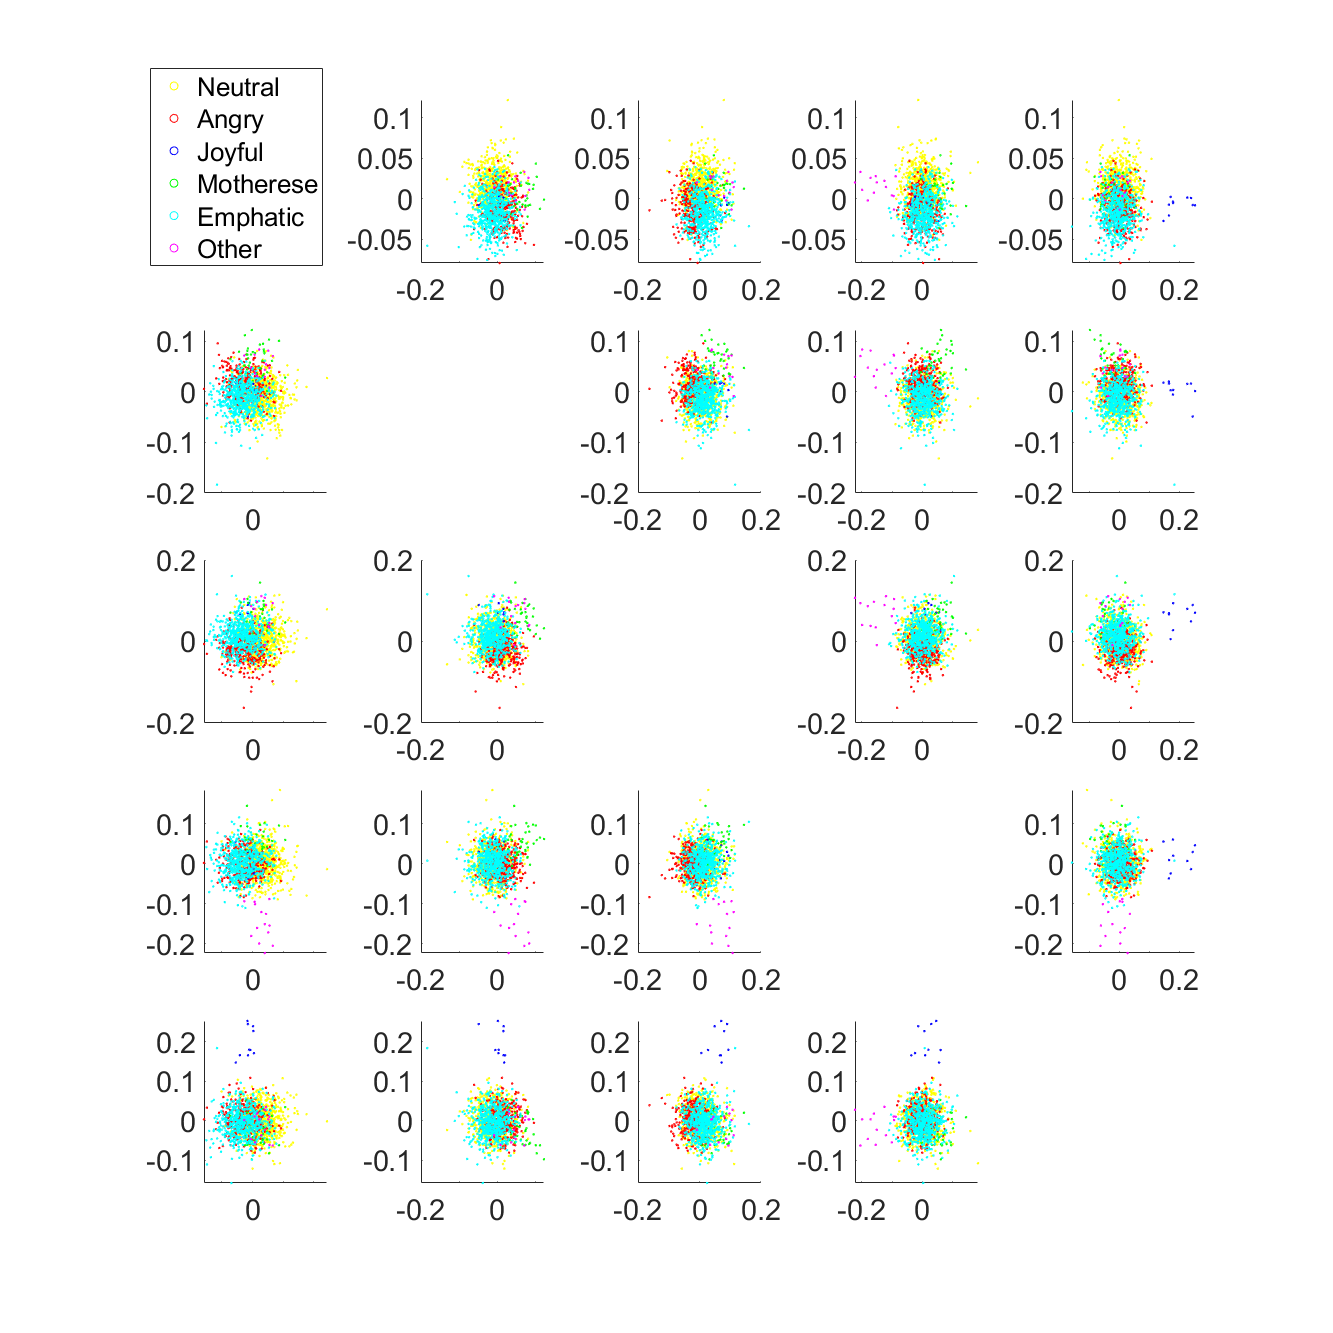
\includegraphics[width=12cm]
			{5graphLDA}}
		\caption{\label{fig:5graphLDA} 2D plot of every dimension in an LDA reduced I Vector}
	\end{figure}

	\section{Nearest Neighbor}
	\subsection{Baseline Performance}
	Originally only cosine similarity was used as a baseline metric. However the data implied by Figure \ref{fig:5graphLDA} could not be captured if the cluster means of the overlapping classes were too similar in direction. More information on these classes can be obtained using the distance to their means rather than direction, so euclidean distance was used as another similarity measure. The increase in performance with distance conveys there is potential in experimenting with an intensity based emotion classifier rather than a distinct equivalence class based emotion classifier as distance most likely relates to similar emotions with varying intensities.
	
	\subsection{Optimizations}
	 	 \begin{table}[!hbt]
	 	\caption{Feature Pramaters and UAR of Cosine Similarity}
	 	\centering
	 	\begin{tabular}{|l|l|l|l|l|l|l|l|l|}
	 		\hline
	 		Frame Length (ms)   & 30   & 20   & 40   & 30   & 30   & 30   & 30   & \textbf{40}   \\ \hline
	 		UBM Components      & 64   & 64   & 64   & 128  & 512  & 64   & 64   & \textbf{512}  \\ \hline
	 		I Vector Dimensions & 100  & 100  & 100  & 100  & 100  & 50   & 200  & \textbf{100}  \\ \hline
	 		Cosine Similarity   & 21\% & 21\% & 23\% & 21\% & 22\% & 20\% & 21\% & \textbf{24\%} \\ \hline
	 	\end{tabular}
	 	\label{featureparams}
	 \end{table}
 
	 \subsection{Feature Extraction Optimizations}
	 Table \ref{featureparams} summarizes parameters tweaked during feature extraction and changes to accuracy using cosine similarity. Shorter frame lengths, usually 20ms to 30ms, are favored in speech processing, yet interestingly performance improved with a longer than usual frame length. Since MFCCs were originally designed for speech recognition tasks, this could indicate emotion data is expressed on a longer frame of speech than language. This could also be the case for children's speech and not only emotional data. The UBM and I Vector parameters are standard. Although using 200 dimensions for the I Vector improved performance, the computation time was drastically higher and unreasonable to test over a longer period of time or with a larger dataset, so the final dimensions used during DNN optimization was 100 dimensions.
	 
	 \section{Neural Network}
	 \subsection{Baseline Performance}
	 \begin{table}[!hbt]
	 	\centering
	 	\caption{Perclass basline accuracy using weighted cross entropy loss function}
	 	\begin{tabular}{|r|c|c|c|c|c|c|}
	 		\hline
	 		\textbf{Class}    & Angry  & Joyful & Motherese & Emphatic & Neutral & Other \\ \hline
	 		\textbf{Accuracy} & 73.6\% & 100\%  & 100\%     & 56.6\%   & 52.7\%  & 100\% \\ \hline
	 	\end{tabular}
 	\label{perclass}
	 \end{table}
	 \subsection{Loss Function}
	 When originally using cross entropy as the loss function, baseline performance for LDA/DNN was approximately 20\%, just above one-sixth, or the ratio of one class to all classes. This was definitely due to the class imbalance negatively impacting cross entropy. Once weighted cross entropy was implemented, the UAR improved drastically, avereging at 77\%. While this is close to 5/6, or the ratio of all but one class, the class imbalance was not the factor as the per-class accuracy was more balanced between the classes. The per-class accuracy is listed in Table \ref{perclass} alongside weights to clarify the effect of weighted cross entropy.
\begin{table}[!hbt]
	\centering
	\caption{Per-parameter Optimization}
	\begin{tabular}{|r|c|c|c|}
		\hline
		Parameter                       & Value                   & UAR  & Baseline Differential \\ \hline
		Basline                         & -                       & 77\% & -                     \\ \hline
		\textit{\textbf{Hidden Layers}} & 2                       & 73\% & -4\%                  \\ \cline{2-4} 
		& 3                       & 63\% & -14\%                 \\ \cline{2-4} 
		& 4                       & 42\% & -25\%                 \\ \hline
		Layer Size                      & \textit{\textbf{20}}    & 78\% & +1\%                  \\ \cline{2-4} 
		& 30                      & 72\% & -5\%                  \\ \cline{2-4} 
		& 50                      & 75\% & -2\%                  \\ \cline{2-4} 
		& 80                      & 76\% & -1\%                  \\ \cline{2-4} 
		& 100                     & 70\% & -7\%                  \\ \hline
		Epoch Count                     & \textit{\textbf{10}}    & 79\% & +2\%                  \\ \cline{2-4} 
		& 50                      & 75\% & -2\%                  \\ \cline{2-4} 
		& 75                      & 74\% & -3\%                  \\ \cline{2-4} 
		& 100                     & 74\% & -3\%                  \\ \hline
		Batch Size                      & 10                      & 44\% & -33\%                 \\ \cline{2-4} 
		& \textit{\textbf{50}}    & 77\% & -                     \\ \cline{2-4} 
		& 75                      & 76\% & -1\%                  \\ \cline{2-4} 
		& 100                     & 76\% & -1\%                  \\ \cline{2-4} 
		& 125                     & 74\% & -3\%                  \\ \hline
		SGD + LR                        & 0.001                   & 73\% & -4\%                  \\ \cline{2-4} 
		& 0.003                   & 77\% & -                     \\ \cline{2-4} 
		& \textit{\textbf{0.006}} & 78\% & +1\%                  \\ \cline{2-4} 
		& 0.009                   & 77\% & -                     \\ \cline{2-4} 
		& 0.03                    & 42\% & -35\%                 \\ \hline
		Adam + LR                       & 0.001                   & 73\% & -4\%                  \\ \cline{2-4} 
		& 0.003                   & 77\% & -                     \\ \cline{2-4} 
		& 0.009                   & 78\% & +1\%                  \\ \cline{2-4} 
		& 0.01                    & 77\% & -                     \\ \cline{2-4} 
		& 0.03                    & 54\% & -23\%                 \\ \hline
		Dropout                         & 0.1                     & 76\% & -1\%                  \\ \cline{2-4} 
		& \textit{\textbf{0.2}}   & 78\% & +1\%                  \\ \hline
	\end{tabular}
\label{optparams}
\end{table}
\clearpage
	 \subsection{Parameter Optimization}
	Epoch count, batch size and learning rate displayed alternate behaviours when layer size, dropout and hidden layer count were at optimized rather than baseline levels. The values with the best differential for the learning based parameters before any optimizations were 30, 10, and 0.001 for Epoch count, batch size and learning rate, respectively. The lower learning rate and increased iterations accounted for the higher layer size and lower dropout at baseline by learning slower but over a longer period of time. Since the latter are architecture based parameters that affect the base architecture of the DNN, changes made to them can propagate to the learning step. Results show it was best to optimize architecture based parameters for this reason. The final most optimal combination is presented in Table \ref{final}
	 \begin{table}[!hbt]
	 	\centering
	 	\caption{Most optimal DNN parameters found}
	 	\begin{tabular}{|r|c|}
	 		\hline
	 		Parameter     & Value       \\ \hline
	 		UAR           & 82\%        \\ \hline
	 		Hidden Layers & 1           \\ \hline
	 		Layer Size    & 20          \\ \hline
	 		Epochs        & 10          \\ \hline
	 		Batch Size    & 50          \\ \hline
	 		Learning Rate & SGD - 0.006 \\ \hline
	 		Feature Size  & LDA - 5 dim \\ \hline
	 		Dropout       & 0.2         \\ \hline
	 	\end{tabular}
 	\label{final}
	 \end{table}